\chapter{LPVisual}
\label{chap:lpvisual}

En \'este cap\'itulo se dar\'a una descripci\'on detallada del visualizador {\tt lpvisual}, el visualizador de {\lpmd}, mostrando las opciones disponibles y la forma en que este visualizador trabaja (posicionamiento de la c\'amara, luces, perspectivas, etc.). Puede encontrar ejemplos en el cap\'itulo~\ref{chap:exa}.

%%%%%%%%%%%%%%%%%%%%%%%%%%%%%%%%%%%%%%%%%%%%%%%%%%%%%%%%%%%%%%%%%
%%%%%%%%%%%%%%%%%%%%%%%%%%%%%%%%%%%%%%%%%%%%%%%%%%%%%%%%%%%%%%%%%
\section{Descripci\'on General}

LPVisual es un proyecto independiente, desarrollado por Felipe Gonz\'alez y Sergio Davis. Consiste en un visualizador basado en OpenGL que permite observar las configuraciones at\'omicas en tiempo real, as\'i como monitorear y graficar propiedades de la configuraci\'on a medida que esta evoluciona.\\


La descarga de \textbf{lpvisual}, se puede realizar a trav\'es de \verb|subversion|, con:

\control{svn co sn://www.gnm.cl/lpmd/lpvisual lpvisual}

Para la instalaci\'on y configuraci\'on refierase directamente a la documentaci\'on del m\'odulo. Cualquier duda o consulta respecto al m\'odulo, contacte directamente a los autores.\\

En la figura~\ref{fig:lpvisual1} podemos apreciar las principales caracter\'isticas del visualizador:
\begin{itemize}
\item En la esquina superior derecha, la ventana principal de simulaci\'on. Aqu\'i se pueden ver los \'atomos en movimiento encerrados en la caja de visualizaci\'on, la cual puede o no tener condiciones de borde peri\'odicas. En la esquina superior derecha de esta pantalla se encuentra el controlador de zoom y de rotaciones, el cual puede ser manejado mediante los click del mouse. Por \'ultimo, los ejes de coordenadas se muestran en una esquina de la caja, los cuales evitan perder el punto de referencia cuando la c\'amara rote.
\item En la esquina superior izquierda encontramos el graficador, el cual acepta interactivamente, al cargar la simulaci\'on, las propiedades que el usuario desee graficar (temperatura, presi\'on, energ\'ia potencia, energ\'ia cin\'etica, energ\'ia total, etc.).
\item En la esquina inferior derecha, se encuentra la ventana de datos de simulaci\'on. Cuando el programa es cargado, el usuario puede elegir qu\'e propiedades desea que sean monitoreadas num\'ericamente en esta ventana. Esto es independiente de las propiedades que est\'en siendo monitoreadas en el archivo de control (ver cap.~\ref{chap:input}).
\item Por \'ultimo, en la esquina inferior izquierda, se encuentra la terminal de texto desde donde se ejecut\'o el programa.
\end{itemize}

\newpage
\begin{figure}[h!]
 \centering
 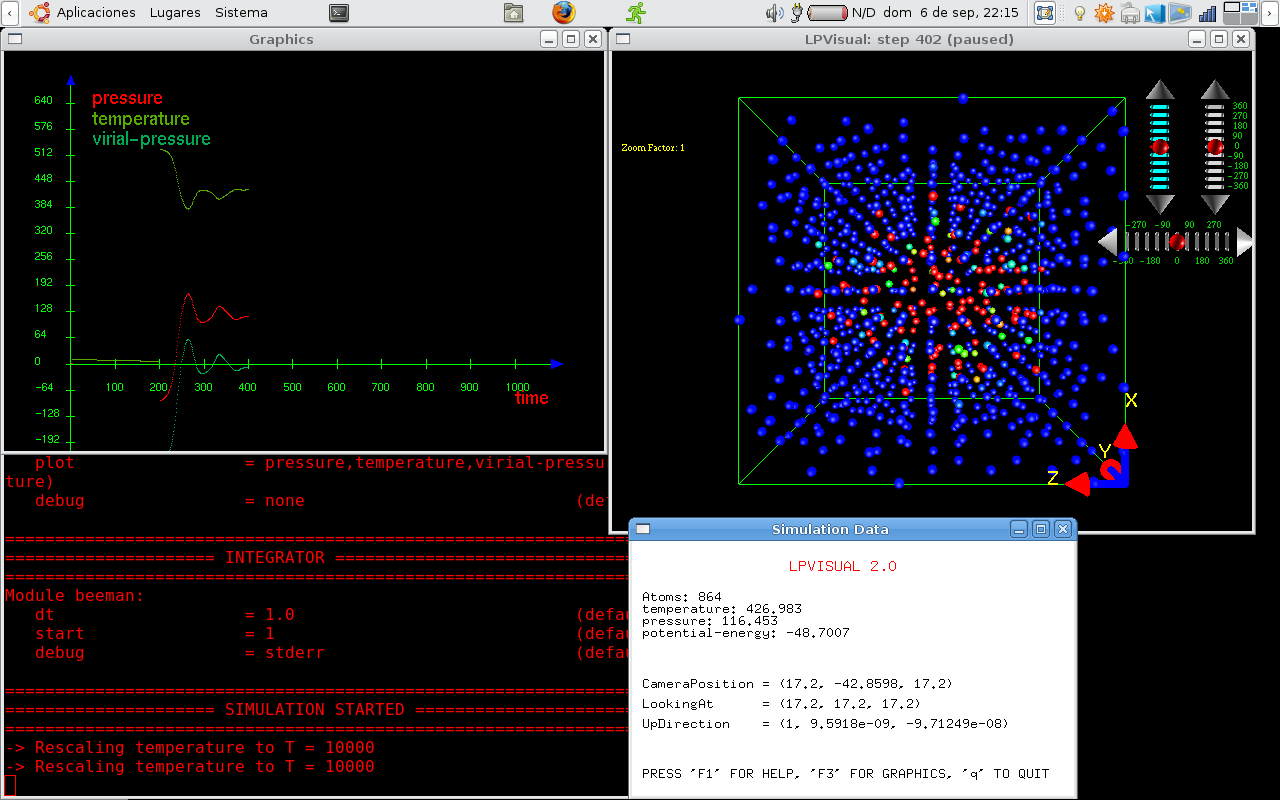
\includegraphics[width=16cm]{lpvisual1.png}
 \caption{Captura de pantalla mientras se ejecuta una simulaci\'on de din\'amica molecular con {\tt lpvisual}.}
 \label{fig:lpvisual1}
\end{figure}


\begin{figure}[h!]
 \centering
 \subfigure{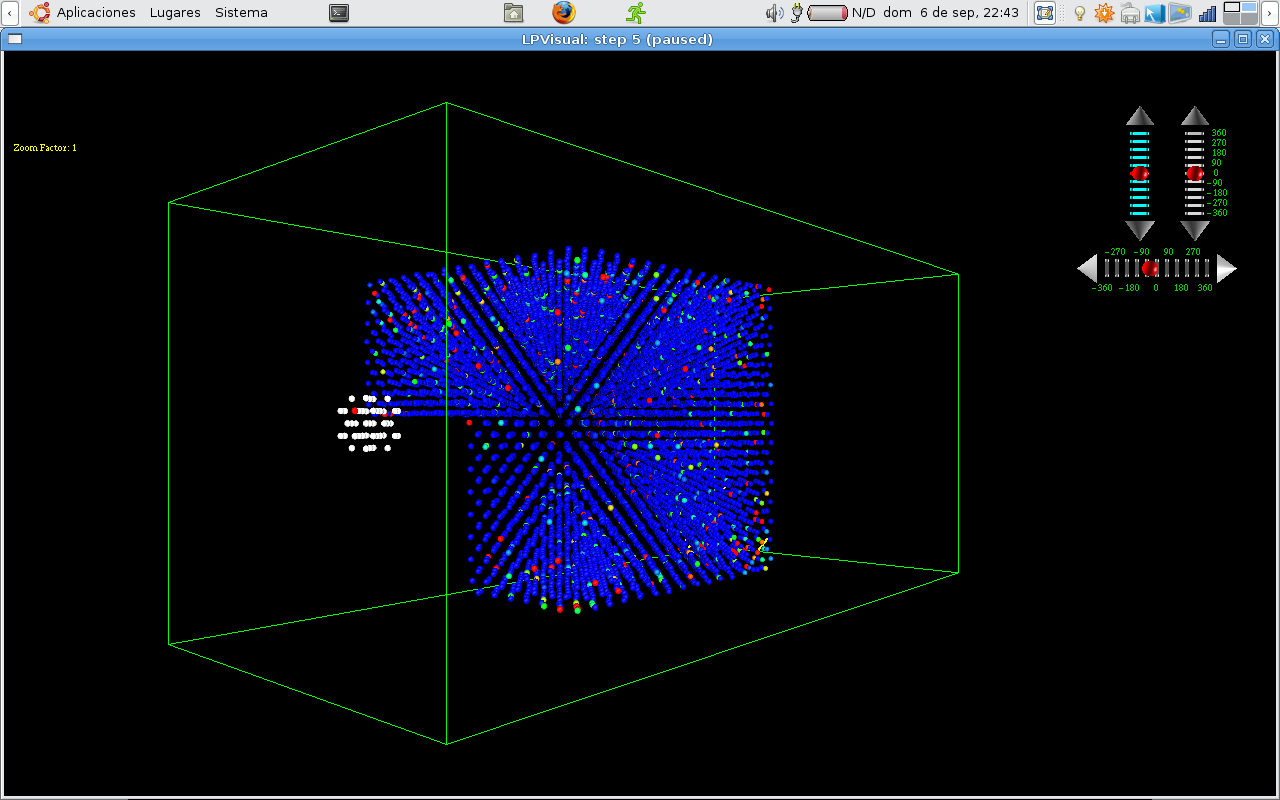
\includegraphics[width=8cm]{lpvisual2.png}}
 \subfigure{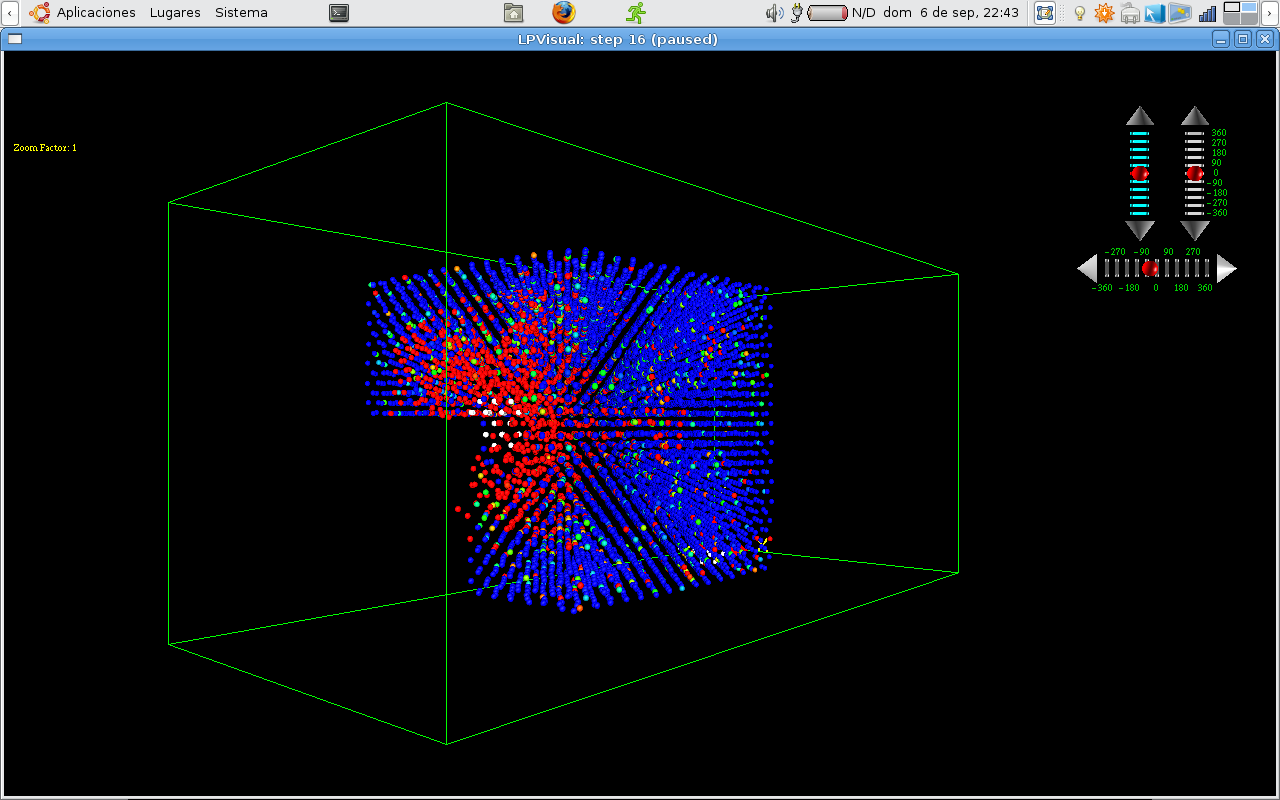
\includegraphics[width=8cm]{lpvisual3.png}}
 \subfigure{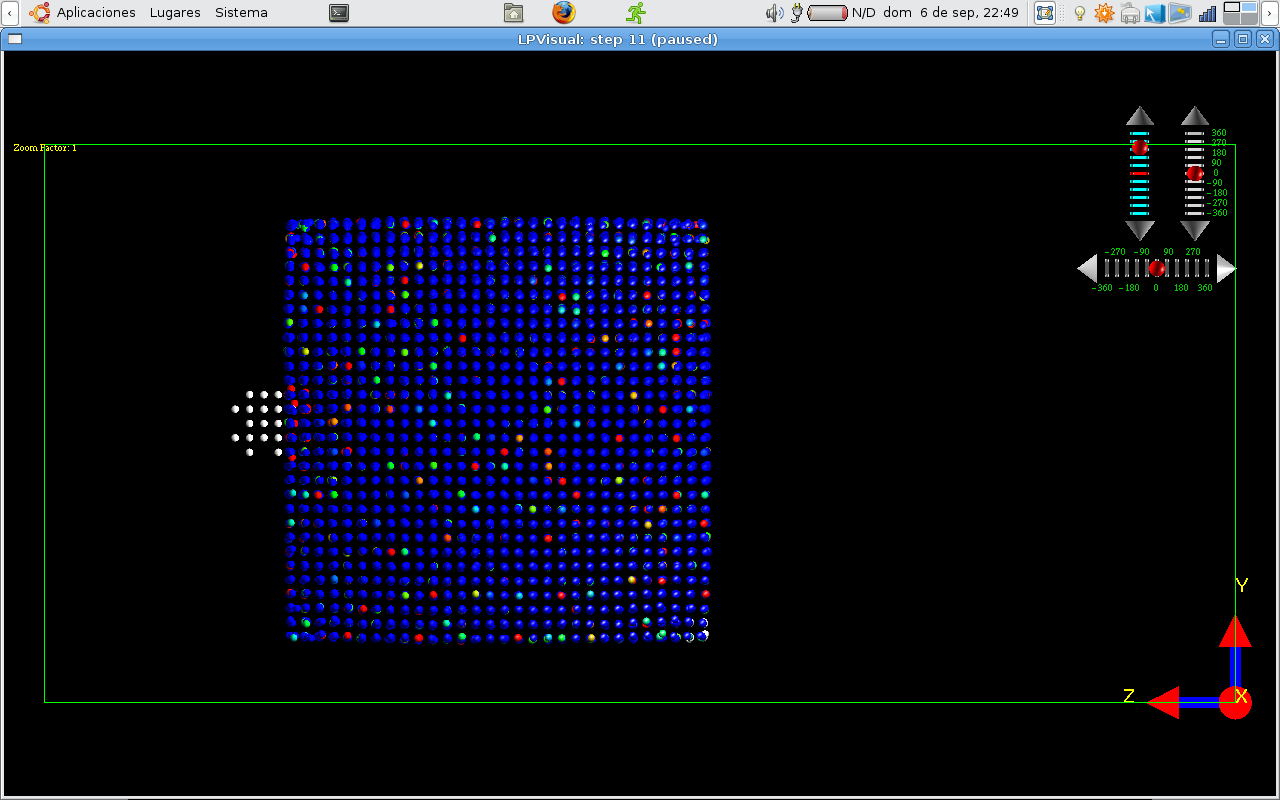
\includegraphics[width=8cm]{lpvisual4.png}}
 \subfigure{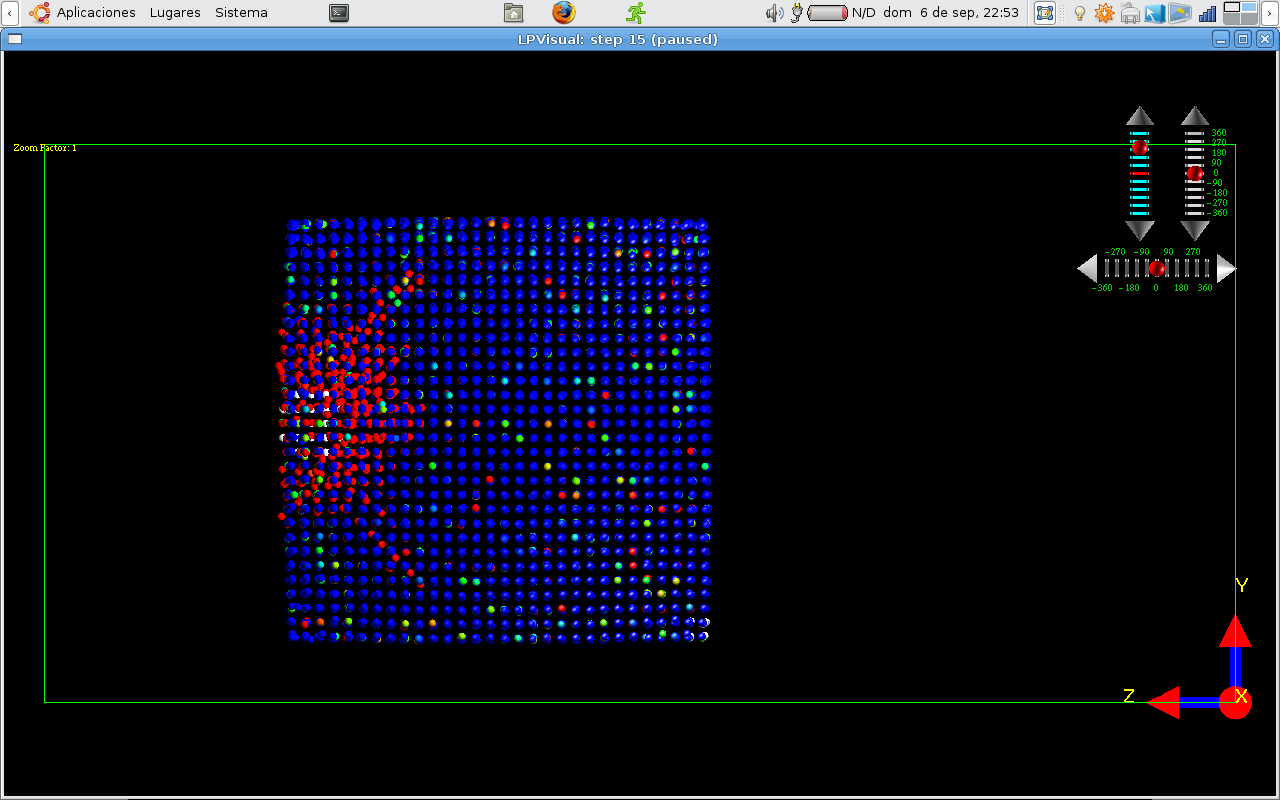
\includegraphics[width=8cm]{lpvisual5.png}}
 \label{fig:lpvisual2}
 \caption{Impacto de un proyectil sobre una celda fcc de 9000 atomos de cobre.}
\end{figure}


\newpage
\subsubsection{Opciones lpvisual}
{\bf lpvisual} ofrece varias opciones durante la visualizaci\'on que son ingresandas tanto del mouse como del teclado:\\

\begin{longtable}[fragile]{|lcp{10.5cm}|}\hline
\multicolumn{3}{|>{\columncolor[rgb]{.45,.45,.45}}c|}{Opciones del Teclado}\\\hline
\tt a&:&Esconde/muestra los ejes de coordenadas.\\
\tt c&:&Esconde/muestra los bordes de la celda de simulaci\'on.\\
\tt f&:&Pantalla completa.\\
\tt F&:&Escala la ventana a su tama\~no original.\\
\tt i&:&Esconde/muestra los controladores zoom y rotaciones.\\
\tt l&:&Cambia los bordes de la celda de simulaci\'on entre placas y espiras.\\
\tt o&:&Selecci\'on de perspectiva (ortogr\'afica / perspectiva).\\
\tt p&:&Pausa.\\
\tt q&:&Salir.\\
\tt r&:&Reset: Deshace rotaciones, movimientos, zoom (restaura la escena).\\
\tt s&:&Activa/desactiva la selecci\'on de \'atomos.\\
\tt t&:&Activa/desactiva la rotaci\'on autom\'atica.\\
\tt z&:&Comienza/detiene el acercamiento.\\
\tt Z&:&Comienza/detiene el alejamiento.\\
\tt +&:&En el modo de selecci\'on de \'atomos, va al \'atomo siguiente.\\
\tt -&:&En el modo de selecci\'on de \'atomos, va al \'atomo anterior.\\
 \tt 1->\tt 9&:&En el modo de selecci\'on de \'atomos, va al \'atomo tipeado (p. ej. ``38'').\\
{\tt CTRL}+{\tt+}&:&Aumenta el factor de zoom (el acercamiento es m\'as r\'apido).\\
{\tt CTRL}+{\tt-}&:&Disminuye el factor de zoom (el acercamiento es m\'as lento).\\
$\bs\uparrow$, $\bs\downarrow$&:&Realizan rotaciones verticales.\\
$\bs\leftarrow$, $\bs\rightarrow$&:&Realizan rotaciones horizontales.\\
{\tt SHIFT}+$\bs\uparrow$, {\tt SHIFT}+$\bs\downarrow$&:&Realizan rotaciones verticales en 5$^o$.\\
{\tt SHIFT}+$\bs\leftarrow$, {\tt SHIFT}+$\bs\rightarrow$&:&Realizan rotaciones horizontales en 5$^o$.\\
{\tt CTRL}+$\bs\uparrow$, {\tt CTRL}+$\bs\downarrow$&:&Realizan traslaciones verticales.\\
{\tt CTRL}+$\bs\leftarrow$, {\tt CTRL}+$\bs\rightarrow$&:&Realizan traslaciones horizontales.\\
{\tt F1}&:&Abre esta ventana.\\
{\tt F2}&:&Abre la ventana de datos de simulaci\'on.\\
{\tt F3}&:&Abre la ventana de gr\'aficos.\\
{\tt RePag}&:&Cambia la fuente de las letras a la pr\'oxima disponible.\\
{\tt AvPag}&:&Cambia la fuente de las letras a la anterior disponible.\\\hline
\multicolumn{3}{|>{\columncolor[rgb]{.45,.45,.45}}c|}{Opciones del Mouse}\\\hline
\multicolumn{1}{|p{4.7cm}}{Click en las flechas horizontales}&:& Rota lentamente la escena horizontalmente.\\
\multicolumn{1}{|p{4.7cm}}{Click en las flechas verticales de la esquina}&:& Rota lentamente la escena verticalmente.\\
\multicolumn{1}{|p{4.7cm}}{Click en las flechas verticales a la izquierda}&:& La camara se acerca o se aleja de la escena.\\\hline
\multicolumn{3}{|>{\columncolor[rgb]{.45,.45,.45}}c|}{Opciones de Movimiento del Mouse}\\\hline
LEFT\_MOUSE\_BUTTON&:& Al presionar esta tecla y mover el mouse simult\'aneamente, permite rotar la celda de simulaci\'on.\\
RIGHT\_MOUSE\_BUTTON&:& Al presionar esta tecla, se desplega el men\'u de la ventana activa.\\
MIDDLE\_MOUSE\_BUTTON&:&Al presionar esta tecla y mover el mouse simult\'aneamente, permite acercar (hacer $zoom$ a) la celda de simulaci\'on.\\\hline
\end{longtable}


